\uuid{s0JY}
\exo7id{5536}
\titre{exo7 5536}
\auteur{rouget}
\organisation{exo7}
\datecreate{2010-07-15}
\isIndication{false}
\isCorrection{true}
\chapitre{Courbes planes}
\sousChapitre{Propriétés métriques : longueur, courbure,...}

\contenu{
\texte{
Déterminer et construire la développée
}
\begin{enumerate}
    \item \question{$\left\{
\begin{array}{l}
x=R\left(\cos t+\ln\left|\tan\frac{t}{2}\right|\right)\\
y=R\sin t
\end{array}
\right.$}
    \item \question{$\left\{
\begin{array}{l}
x=R(t-\sin t)\\
y=R(1-\cos t)
\end{array}
\right.$.}
    \item \question{$y=x^3$}
\reponse{
On obtient la courbe complète quand $t$ décrit $]-\pi,0[\cup]0,\pi[$. Puisque $M(-t)=s_{(Ox)}(M(t))$ et $M(\pi-t)=s_{(Oy)}(M(t))$, on se contente d'étudier et de construire la courbe quand $t\in\left]0,\frac{\pi}{2}\right[$ puis on obtient la courbe complète par réflexions successives d'axe $(Oy)$ puis d'axe $(Ox)$.
Pour $t\in\left]0,\frac{\pi}{2}\right[$,

\begin{center}
$\overrightarrow{\frac{dM}{dt}}=\left(
\begin{array}{c}
R(-\sin t+\frac{1}{\sin t})\\
R\cos t
\end{array}
\right)=R\left(
\begin{array}{c}
\frac{\cos^2t}{\sin t}\\
\cos t
\end{array}
\right)=R\frac{\cos t}{\sin t}\left(
\begin{array}{c}
\cos t\\
\sin t
\end{array}
\right)=R\cotan t\left(
\begin{array}{c}
\cos t\\
\sin t
\end{array}
\right).$
\end{center}
Puisque $R\cotan t>0$ pour $t\in\left]0,\frac{\pi}{2}\right[$ et puisque le vecteur $\left(
\begin{array}{c}
\cos t\\
\sin t
\end{array}
\right)$ est unitaire, on a

\begin{center}
$\frac{ds}{dt}=R\cotan t$ puis $\overrightarrow{\tau}(t)=\left(
\begin{array}{c}
\cos t\\
\sin t
\end{array}
\right)$.
\end{center}
On a donc $\overrightarrow{n}(t)=\left(
\begin{array}{c}
-\sin  t\\
\cos t
\end{array}
\right)$ et d'autre part, on peut prendre $\alpha(t)=t$. En notant $\rho(t)$ le rayon de courbure au point $M(t)$,

\begin{center}
$\rho(t)=\frac{ds}{d\alpha}=\frac{ds/dt}{d\alpha/dt}=R\cotan t$,
\end{center}
puis

\begin{align*}\ensuremath
\Omega(t)&=M(t)+\rho(t)\overrightarrow{n}(t)=\left(
\begin{array}{c}
R\left(\cos t+\ln\left|\tan \frac{t}{2}\right|\right)\\
R\sin t
\end{array}
\right)+R\cotan t\left(
\begin{array}{c}
-\sin  t\\
\cos t
\end{array}
\right)\\
 &=\left(
\begin{array}{c}
R\ln\left|\tan \frac{t}{2}\right|\\
\frac{R}{\sin t}
\end{array}
\right).
\end{align*}
La développée cherchée est l'arc $t\mapsto\left(
\begin{array}{c}
R\ln\left|\tan \frac{t}{2}\right|\\
\frac{R}{\sin t}
\end{array}
\right)$, $t\in]-\pi,0[\cup]0,\pi[$ (en complétant par symétrie). Quand $t$ décrit $]0,\pi[$, on effectue alors le changement de paramètres $t\mapsto R\ln\left|\tan \frac{t}{2}\right|=u$ qui est un $C^1$-difféomorphisme de $]0,\pi[$ sur $\Rr$. On obtient $x=u$ puis

\begin{center}
$y=\frac{R}{\frac{2\tan\frac{t}{2}}{1+\tan^2\frac{t}{2}}}=\frac{R}{2}\left(\tan\frac{t}{2}+\frac{1}{\tan\frac{t}{2}}\right)=R\frac{e^{u/R}+e^{-u/R}}{2}=R\ch\left(\frac{u}{R}\right)$.
\end{center}
Le support de la développée sur $]0,\pi[$ est aussi le support de l'arc $u\mapsto\left(
\begin{array}{c}
u\\
R\ch\left(\frac{u}{R}\right)
\end{array}
\right)$, $u\in\Rr$ ou encore la chaînette d'équation cartésienne $y=R\ch\left(\frac{x}{R}\right)$.

$$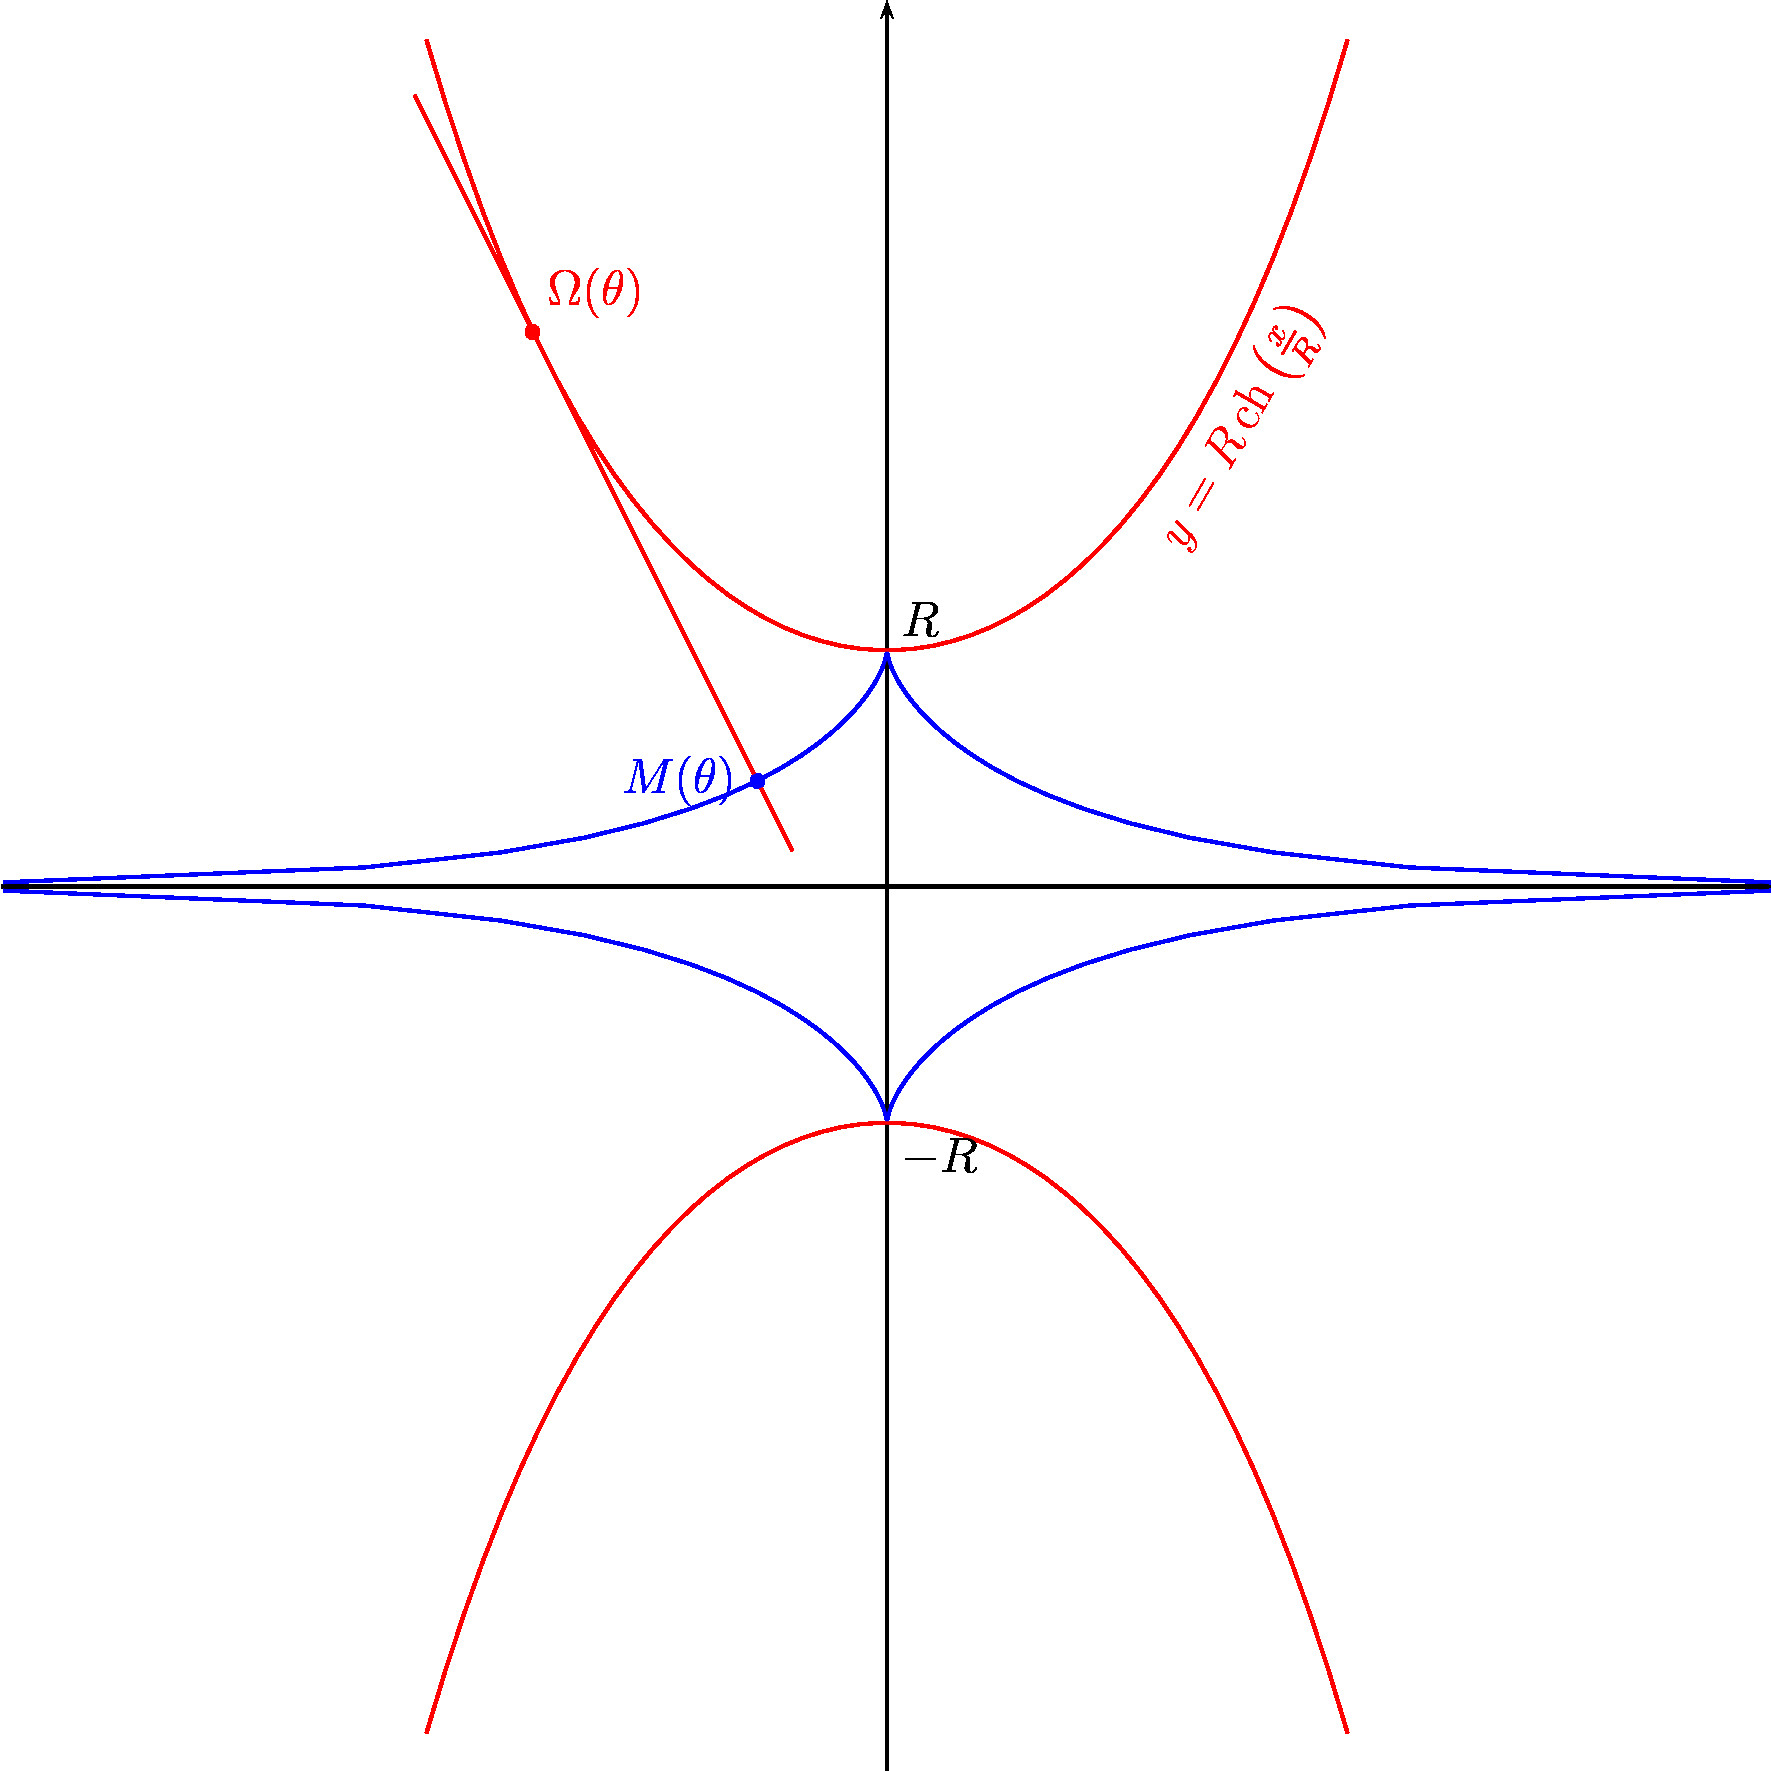
\includegraphics{../images/img005536-1}$$

 \item  Quand $t$ décrit $[0,2\pi]$, on obtient une arche de cycloïde complète. Les autres arches s'en déduisent par translations de vecteurs $2k\pi R\overrightarrow{i}$. Pour $t\in[0,2\pi]$

\begin{center}
$\overrightarrow{\frac{dM}{dt}}=\left(
\begin{array}{c}
R(1-\cos t)\\
R\sin t
\end{array}
\right)=2R\sin\left(\frac{t}{2}\right)\left(
\begin{array}{c}
\sin\left(\frac{t}{2}\right)\\
\rule{0mm}{6mm}\cos\left(\frac{t}{2}\right)
\end{array}
\right).$
\end{center}
Le point $M(t)$ est régulier pour $t\in]0,2\pi[$ et pour $t\in]0,2\pi[$, $2R\sin\left(\frac{t}{2}\right)>0$. Puisque le vecteur $\left(
\begin{array}{c}
\sin\left(\frac{t}{2}\right)\\
\rule{0mm}{6mm}\cos\left(\frac{t}{2}\right)
\end{array}
\right)$ est unitaire, on a

\begin{center}
$\frac{ds}{dt}=2R\sin\left(\frac{t}{2}\right)$ et $\overrightarrow{\tau}(t)=\left(
\begin{array}{c}
\sin\left(\frac{t}{2}\right)\\
\rule{0mm}{6mm}\cos\left(\frac{t}{2}\right)
\end{array}
\right)=\left(
\begin{array}{c}
\cos\left(\frac{\pi}{2}-\frac{t}{2}\right)\\
\rule{0mm}{6mm}\sin\left(\frac{\pi}{2}-\frac{t}{2}\right)
\end{array}
\right)$.
\end{center}
On en déduit que $\overrightarrow{n}(t)=\left(
\begin{array}{c}
-\cos\left(\frac{t}{2}\right)\\
\rule{0mm}{6mm}\sin\left(\frac{t}{2}\right)
\end{array}
\right)$ et d'autre part, on peut prendre $\alpha(t)=\frac{\pi}{2}-\frac{t}{2}$. En notant $\rho(t)$ le rayon de courbure au point $M(t)$,

\begin{center}
$\rho(t)=\frac{ds}{d\alpha}=\frac{ds/dt}{d\alpha/dt}=\frac{2R\sin\left(\frac{t}{2}\right)}{-\frac{1}{2}}=-4R\sin\left(\frac{t}{2}\right)$,
\end{center}
et donc

\begin{align*}\ensuremath
\Omega(t)&=M(t)+\rho(t)\overrightarrow{n}(t)=\left(
\begin{array}{c}
R(t-\sin t)\\
R(1-\cos t)
\end{array}
\right)-4R\sin\left(\frac{t}{2}\right)\left(
\begin{array}{c}
-\cos\left(\frac{t}{2}\right)\\
\rule{0mm}{6mm}\sin\left(\frac{t}{2}\right)
\end{array}
\right)=\left(
\begin{array}{c}
R(t-\sin t)+2R\sin t\\
R(1-\cos t)-2R(1-\cos t)
\end{array}
\right)\\
 &=\left(
\begin{array}{c}
R(t+\sin t)\\
-R(1-\cos t)
\end{array}
\right).
\end{align*}
La développée cherchée est l'arc $t\mapsto\left(
\begin{array}{c}
R(t+\sin t)\\
-R(1-\cos t)
\end{array}
\right)$. Poursuivons.

\begin{align*}\ensuremath
\Omega(t+\pi)&=\left(
\begin{array}{c}
R(t+\pi-\sin t)\\
-R(1+\cos t)
\end{array}
\right)=\left(
\begin{array}{c}
R(t-\sin t)\\
R(1-\cos t)
\end{array}
\right)+\left(
\begin{array}{c}
\pi R\\
-2R
\end{array}
\right)=t_{\overrightarrow{u}}(M(t))\;\text{où}\;\overrightarrow{u}=(\pi R,-2R).
\end{align*}
Ainsi, le centre de courbure au point $M(t+\pi)$ est le translaté du point $M(t)$ dans la translation de vecteur $(\pi R,-2R)$ et donc la développée de la cycloïde est la translatée de la cycloïde par la translation de vecteur $(\pi R,-2R)$. En particulier, c'est encore une cycloïde.

$$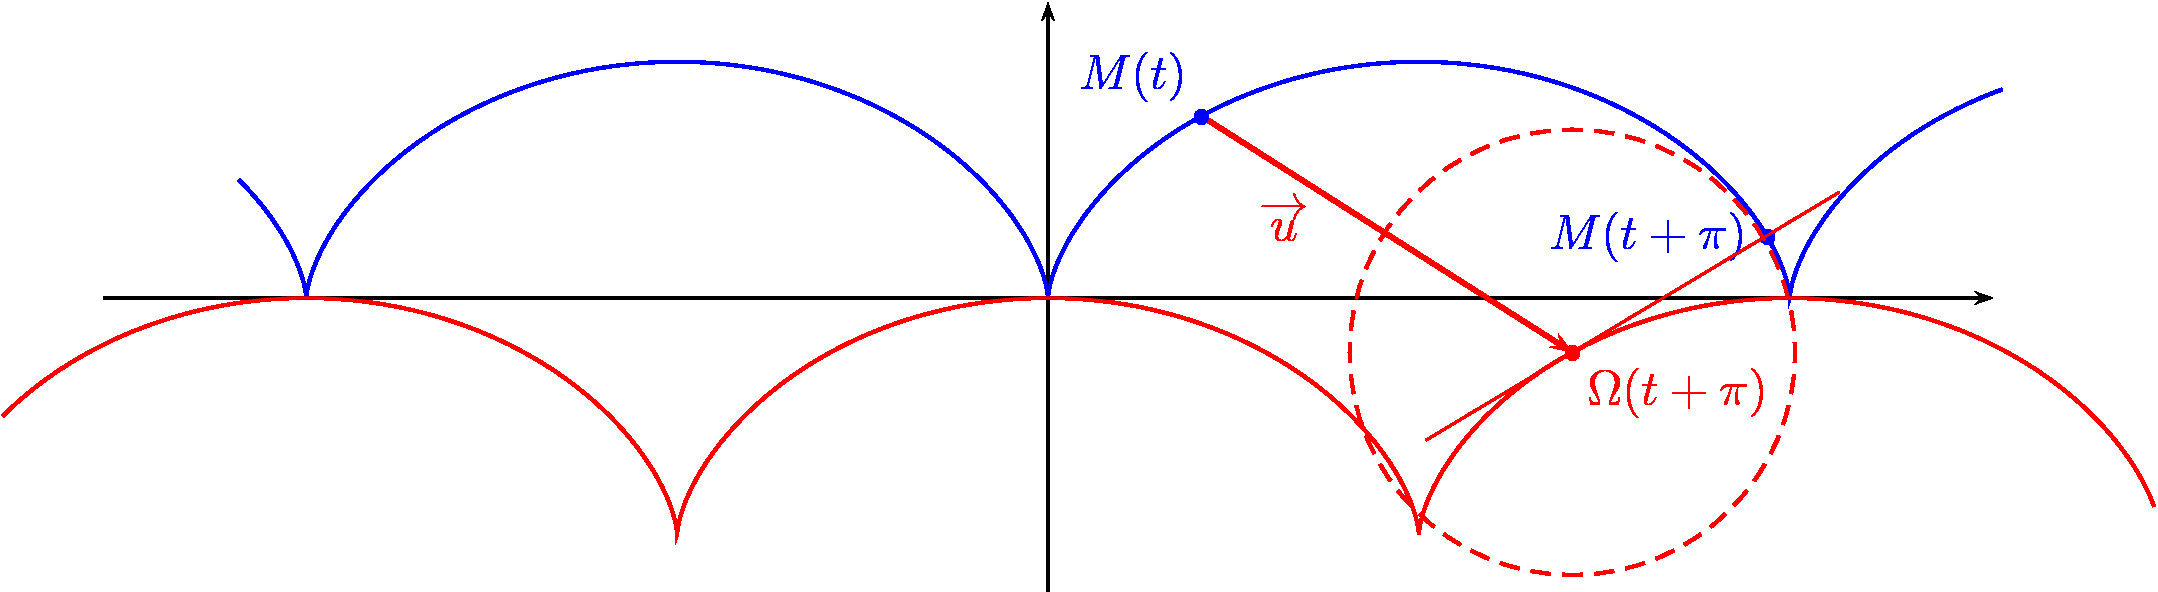
\includegraphics{../images/img005536-2}$$

 \item  $\mathcal{C}$ est le support de la courbe paramétrée $t\mapsto M(t)=\left(
\begin{array}{c}
t\\
t^3
\end{array}
\right)$. $M(t)$ est birégulier si et seulement si $t/neq0$. Pour $t\in\Rr$, $\overrightarrow{\frac{dM}{dt}}=\left(
\begin{array}{c}
1\\
3t^2
\end{array}
\right)$. Par suite 

\begin{center}
$\frac{ds}{dt}=\sqrt{1+9t^4}$ et $\overrightarrow{\tau}(t)=\frac{1}{\sqrt{1+9t^4}}\left(
\begin{array}{c}
1\\
3t^2
\end{array}
\right)$.
\end{center}
Donc, d'une part $\overrightarrow{n}(t)=\frac{1}{\sqrt{1+9t^4}}\left(
\begin{array}{c}
-3t^2\\
1
\end{array}
\right)$ et d'autre part, puisque les coordonnées de $\overrightarrow{\tau}(t)$ sont positives, on peut prendre $\alpha(t)=\Arccos\left(\frac{1}{\sqrt{1+9t^4}}\right)$. Par suite, pour $t\neq0$

\begin{center}
$\frac{d\alpha}{dt}=-\left(-\frac{1}{2}\right)36t^3(1+9t^4)^{-3/2}\times\frac{1}{\sqrt{1-\frac{1}{1+9t^4}}}=\frac{6t}{1+9t^4}$
\end{center}
puis

\begin{center}
$R(t)=\frac{ds/dt}{d\alpha/dt}=\frac{(1+9t^4)^{3/2}}{6t}$,
\end{center}
et donc

\begin{center}
$\Omega(t)=M(t)+R(t)\overrightarrow{n}(t)=\left(
\begin{array}{c}
t\\
t^3
\end{array}
\right)+
\frac{1+9t^4}{6t}\left(
\begin{array}{c}
-3t^2\\
1
\end{array}
\right)
=\left(
\begin{array}{c}
\frac{t}{2}-\frac{9t^5}{2}\\
\rule{0mm}{6mm}\frac{5t^3}{2}+\frac{1}{6t}
\end{array}
\right)$.
\end{center}

$$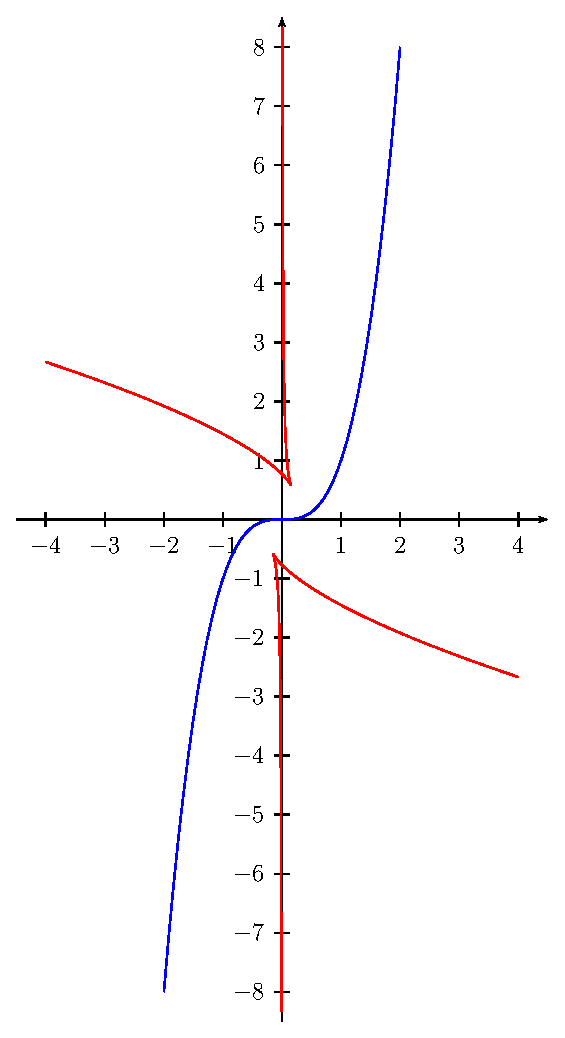
\includegraphics{../images/img005536-3}$$
}
\end{enumerate}
}
